\section{Simulation Environment}
\label{sec:methodology-simulation-environment}

\begin{outline}
  Describe the physics-based simulation environment (IsaacLab) and
  the quadruped model used for development and testing.
\end{outline}

The simulation environment used for this project is NVIDIA Isaac Lab
\cite{mittal_orbit_2023}. This framework was selected for several
reasons. It is a modern platform with a Python interface designed
specifically for RL applications and GPU parallelism. The use of GPU
parallelism enables significantly faster simulation and data
collection, albeit at the cost of increased programming complexity
and reduced compatibility with older hardware. Furthermore, the
extensive collection of example and community projects provides
valuable references for implementing the simulation features required
in this work.

Although both simulation and learning processes are executed on the
GPU, the robot controllers operate on the CPU.
\autoref{fig:diagram-processing-flow} illustrates the overall
processing flow. The simulation environment runs entirely on the GPU,
where multiple robots are simulated in parallel. Meanwhile, the robot
MPCs execute on the CPU, with each controller running concurrently.
The CPU and GPU communicate at every simulation step to exchange
robot states and corresponding control actions.

\begin{figure}[H]
  \centering
  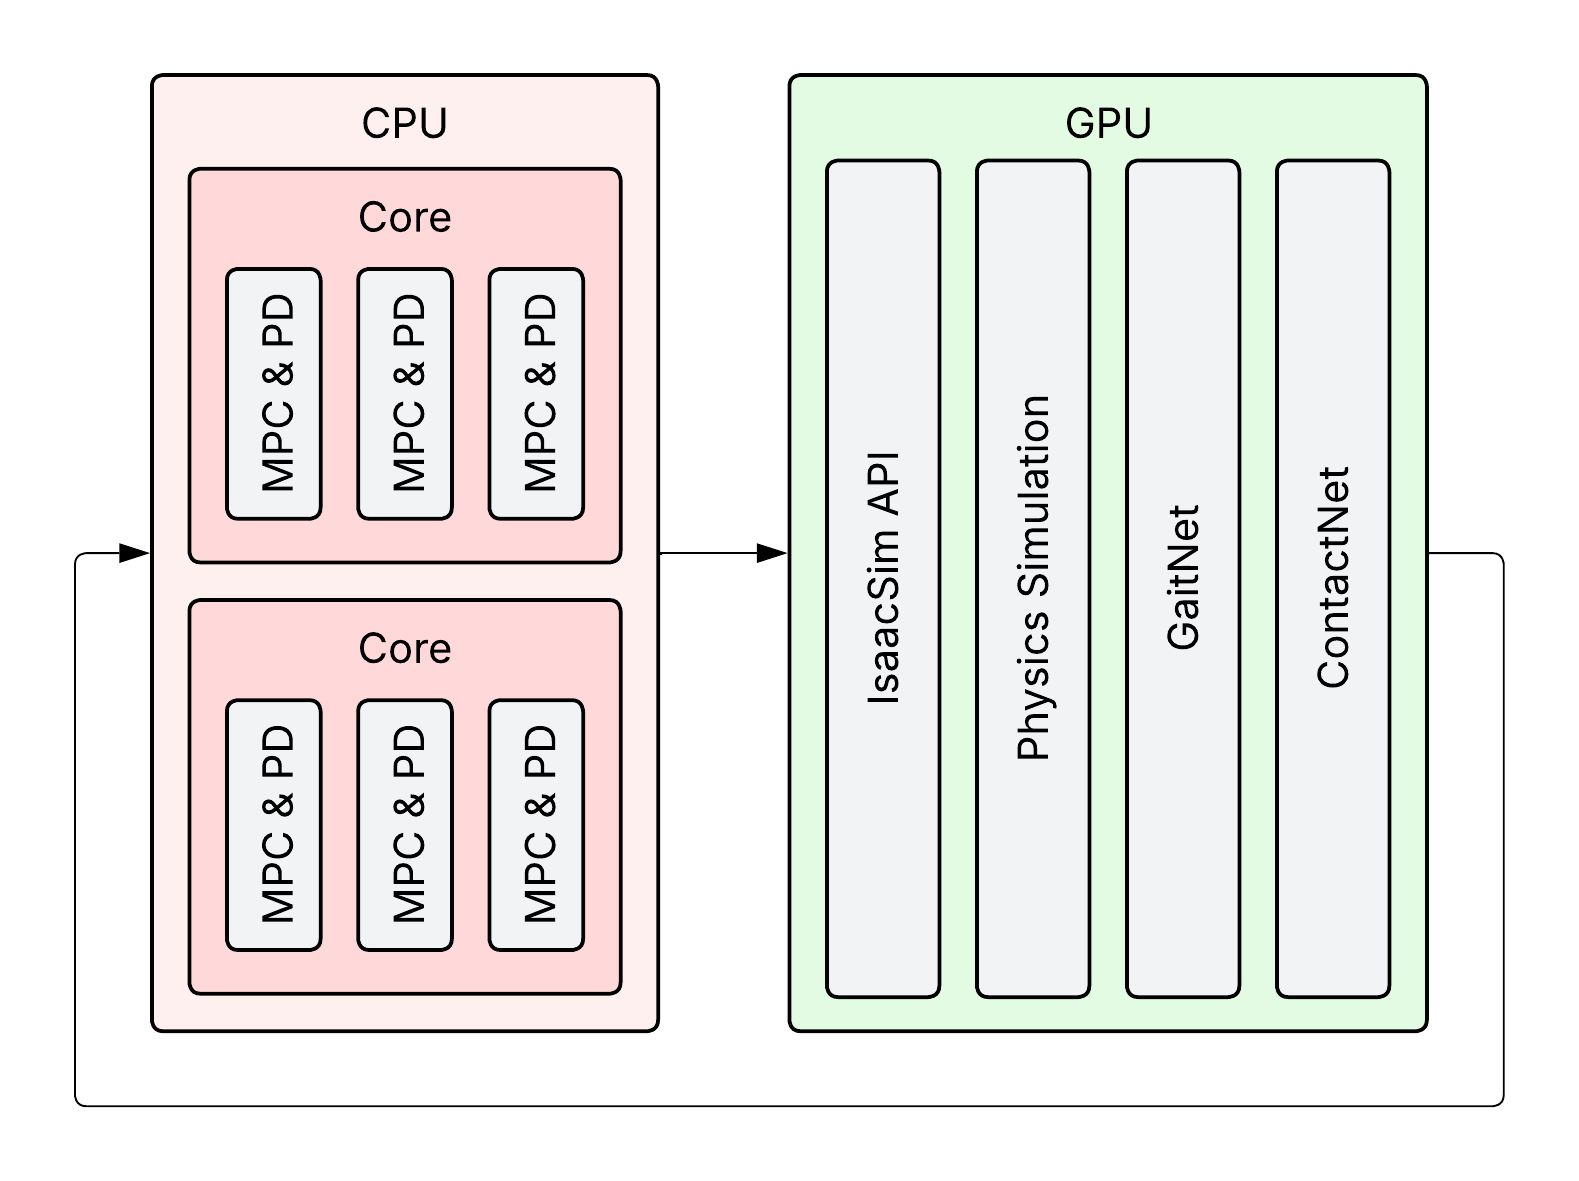
\includegraphics[width=0.5\linewidth]{images/diagrams/processing-flow.png}
  \caption{A block diagram showing the programming tasks computed on
    the CPU vs GPU. The full simulation is run in parallel using Nvidia
  Isaac Lab on the GPU, while the robot MPCs are run in parallel on the CPU.}
  \label{fig:diagram-processing-flow}
\end{figure}

NVIDIA Isaac Lab uses a declarative system of python dataclasses to
define the simulation environment. For this work, a custom
environment is used (\autoref{fig:figure-envirnment-close}), including:

\begin{itemize}
  \item Unitree Go 1\textemdash Configured to use force control for each joint.
  \item Terrain raycasts\textemdash Measure the height of the terrain
    at each possible footstep location. This emulates the lidar
    processing steps of a full vision pipeline.
  \item Custom terrain\textemdash Planar terrain with sections
    missing on a grid pattern. The underlying grid is 12\,cm square,
    and the void density varying from $\sim$0\% to 40\%. Multiple
    difficulty levels of the     terrain are generated for the robots
    to progress through as     they learn. The terrain is designed to
    mirror that used in
    \cite{bratta_contactnet_2024}. A view of the full terrain is shown
    in \autoref{fig:figure-envirnment-far}.
\end{itemize}

\begin{figure}[H]
  \centering
  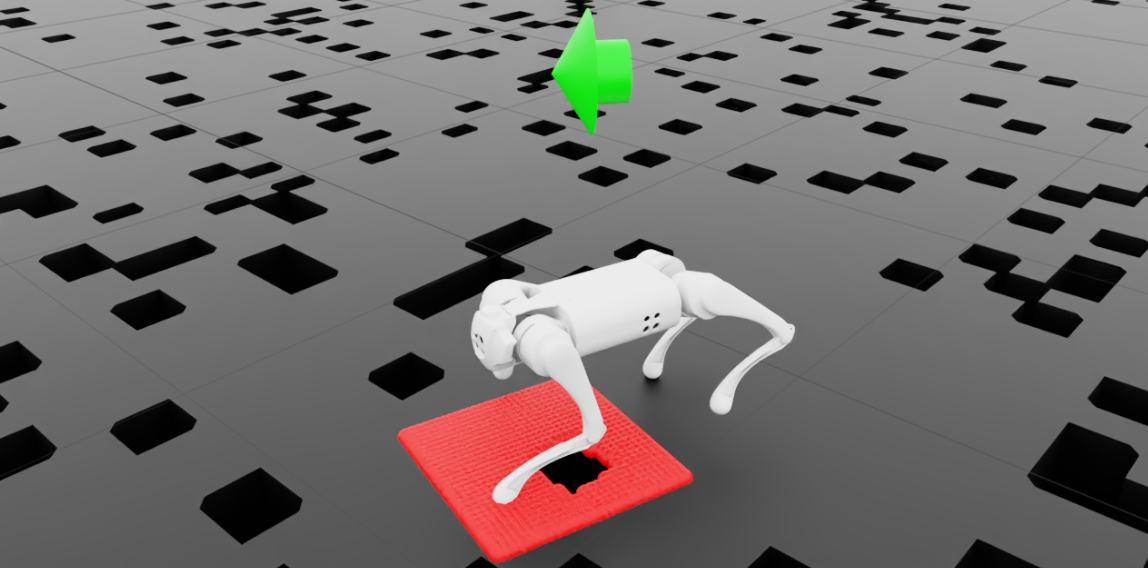
\includegraphics[width=0.75\linewidth]{images/figures/environment-close.png}
  \caption{Image of a Unitree Go 1 navigating the terrain. Red
    region shows area converted into heightmap for front left leg.
    Black regions show voids   in the terrain. Green arrow shows
  desired velocity vector.}
  \label{fig:figure-envirnment-close}
\end{figure}

\begin{figure}[H]
  \centering
  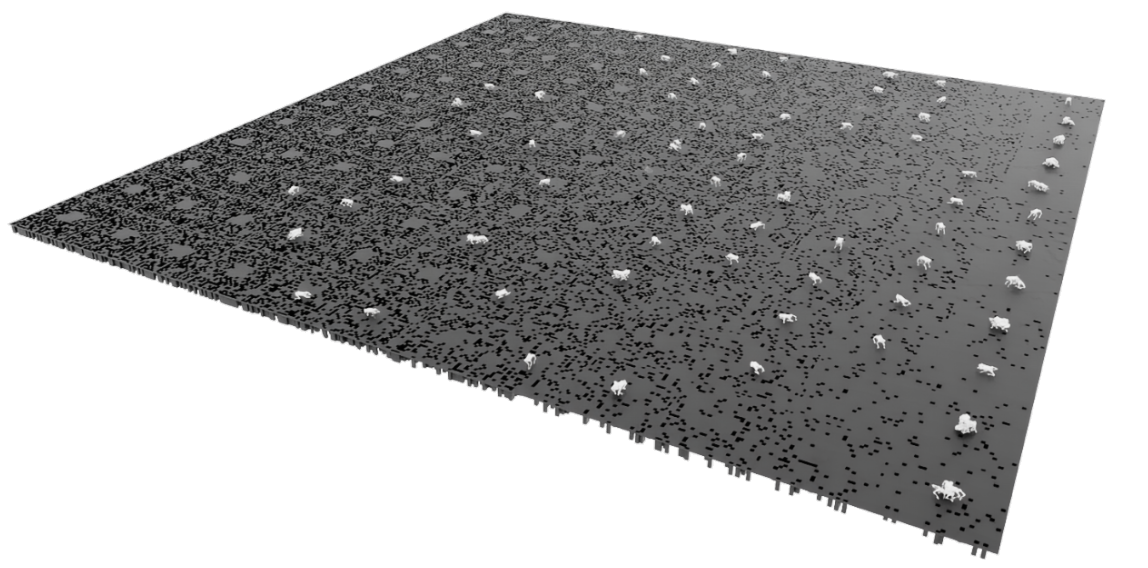
\includegraphics[width=0.75\linewidth]{images/figures/environment-far.png}
  \caption{Image showing the full terrain used in simulation.
    Full terrain is a grid of 12x12 sub-terrains with increasing
  difficulty.     Sub-terrains are 4x4\,m grids with missing sections.}
  \label{fig:figure-envirnment-far}
\end{figure}
